\documentclass[11pt]{article}

\usepackage[margin=1in]{geometry}
\usepackage{amsmath,amssymb,amsthm}
\newtheorem{proposition}{Proposition}
\usepackage{booktabs}
\usepackage{graphicx}
\usepackage{microtype}
\usepackage{float}
\usepackage{caption}
\usepackage{subcaption}
\usepackage{xcolor}
\usepackage[round]{natbib}
\usepackage[hidelinks]{hyperref}
\usepackage{enumitem}
\usepackage{array}

\graphicspath{{figures/}{../artifacts/}}
\setlength{\parskip}{0.4em}
\setlength{\parindent}{0pt}
\setlist{nosep}
\captionsetup{font=small}

\newcommand{\code}[1]{\texttt{#1}}
\newcommand{\doi}[1]{\href{https://doi.org/#1}{doi:#1}}
\newcommand{\E}{\mathbb{E}}
\newcommand{\Prb}{\mathop{\mathrm{Pr}}}
\newcommand{\Normal}{\mathcal{N}}

% Visible placeholder for biologist coauthors to complete. Statistical-modeling
% sections are drafted; biology/ecology pieces are flagged like this.
\newcommand{\needbio}[1]{%
  \par\smallskip\noindent%
  \textcolor{purple}{$\blacktriangleright$~\textbf{[COAUTHOR INPUT NEEDED~--~biology/ecology]:}\space\textit{#1}}%
  \par\smallskip}

\title{\bfseries What Can Repeated Size Profiles Identify?\\
Bayesian Inference and Confounding in Inverse Integral Projection Models}

\author{%
  Robert Richardson\thanks{Corresponding author. Department of Statistics.
  Statistical modeling, inference, and writing.}\\
  \textcolor{purple}{[Biologist coauthors to be added]}}

\date{\today}

\begin{document}
\maketitle

\begin{abstract}
\noindent
Repeated cross-sectional size profiles---counts of individuals by body
size collected over several years---are among the most common and least
expensive data in population ecology. It is tempting to invert a size-structured
integral projection model (IPM) against such data and read off survival, growth,
and reproduction. We ask instead a prior question: \emph{which} vital rates are
identified by repeated profiles, which are confounded, and what additional
information resolves them. Using an individual-based generator distinct from the
recovery model, a positive numerical-quadrature inverse IPM, and a fully Bayesian
treatment, we show that size profiles reliably recover survival, the growth
increment, and the recruit-size distribution, but that recruitment intensity is
only weakly identified, along a single ridge in parameter space. We prove two
identifiability results---a decomposition result (the total per-capita
contribution of each size is identified but its split into survival and
recruitment is not, wherever growth and recruit sizes overlap) and an excitation
result (near a stable size distribution, profiles constrain the asymptotic growth
rate $\lambda$ and the stable shape far more tightly than the vital rates that
generate them)---and confirm both numerically. We calibrate the posterior
approximation by simulation-based calibration, quantify how size-dependent
detection corrupts recovery, and measure how much auxiliary individual-level data
are required to break the confounding. A 20-year brook trout capture--mark--recapture study illustrates the
central caution: a profile-only fit can look entirely plausible yet badly
misestimate growth and the size pattern of survival, which only the individual
data reveal. We frame the contribution as a diagnostic framework---what is
identified, how to detect confounding, and how to design the data or priors
needed for credible inference---rather than a claim that profiles generally
identify vital rates.
\end{abstract}

\noindent\textbf{Keywords:} integral projection models; identifiability;
inverse problems; Bayesian hierarchical models; integrated population models;
simulation-based calibration; size-structured populations.

\section{Introduction}
\label{sec:intro}

Size-structured populations are routinely monitored by repeated cross-sectional
surveys that record the body sizes of sampled individuals. The resulting
\emph{size profiles}---histograms of size at successive census times---are
inexpensive relative to individual marking, and they exist for many taxa over
long periods. The integral projection model
\citep{easterling2000,ellner2006,merow2014} provides a natural mechanistic
description of how such a profile should evolve: a kernel built from
size-dependent survival, growth, and reproduction maps this year's size
distribution to next year's. A seemingly direct strategy is therefore to invert
the IPM against repeated profiles and recover the vital-rate functions. This is
an instance of a classic inverse problem for structured populations
\citep{wood1994,gross2002,ghosh2012}, and like most inverse problems it is
ill-posed: many different vital-rate configurations can generate nearly identical
profile dynamics.

The central message of this paper is that the correct scientific question is not
``can we fit an inverse IPM to size profiles'' (we almost always can) but
``\emph{what does the fit identify}.'' A model can reproduce observed profile
dynamics accurately while estimating a population-effective transition operator
that differs from the individual vital rates that generated the data, and it can
report narrow posterior intervals that are an artifact of the prior rather than
the data. We therefore treat identifiability, confounding, and prior sensitivity
as first-class objects of study, declare the estimands before fitting, and
validate recovery against data generated by a process \emph{other} than the
recovery model.

Our contributions are: (i) a clean separation of an individual-based biological
generator from the recovery model, so that the inverse IPM is never validated
only on data from the same IPM; (ii) a decomposition of which vital rates are
identified by repeated profiles and a characterization---analytical and
numerical---of the confounding ridge between recruitment intensity and its
size gradient; (iii) a calibrated Bayesian workflow, including
simulation-based calibration of the posterior approximation and an explicit
demonstration that size-dependent detection, if unmodeled, is mistaken for
demography; (iv) a quantitative account of how much auxiliary individual data
break the confounding, including robust prior borrowing and its transportability
limits; and (v) a real-data application to a long brook trout time series in
which profile-only inference is benchmarked against capture--mark--recapture and
integrated analyses. The methodological emphasis and the identifiability
diagnostics are intended to be portable to other size- or stage-structured
inverse problems.

\needbio{One to two paragraphs of ecological and management motivation:
why size profiles are collected in your systems, what management or conservation
decisions rest on vital-rate estimates from them, and why distinguishing
identified from confounded rates matters in practice. Cite the key applied
literature for the focal taxa.}

The remainder of the paper declares the estimands and notation
(Section~\ref{sec:estimands}), specifies the generator, observation process,
recovery model, priors, inference, and diagnostics (Section~\ref{sec:methods}),
reports the simulation experiments (Section~\ref{sec:sim}), presents the brook
trout application (Section~\ref{sec:app}), and discusses scope and limitations
(Section~\ref{sec:discussion}).

\section{Estimands and Notation}
\label{sec:estimands}

We distinguish four inferential targets and report them separately throughout,
because good performance on one does not imply recovery of another:
\begin{enumerate}
  \item \textbf{Individual vital rates:} survival probability $s(x)$, mean and
  spread of the growth transition $g(x'\mid x)$, realized recruitment intensity
  $r(x)$, and the recruit-size distribution $b(x'\mid x)$, as functions of
  individual size $x$.
  \item \textbf{Population-effective rates:} the same quantities after averaging
  over unobserved heterogeneity, movement, and detection---what a size-only model
  can at best target.
  \item \textbf{Kernel functionals:} the dominant eigenvalue $\lambda$ (asymptotic
  population growth rate), the stable size distribution, and sensitivities.
  \item \textbf{Prediction targets:} next-year and multi-year size profiles.
\end{enumerate}
Throughout, $x$ denotes size on a fixed mesh, $\Delta x$ the mesh spacing,
$\boldsymbol{\mu}_t$ the latent population size-intensity at census $t$, and
$Y_{tj}$ the observed count in size bin $j$ at census $t$.

\section{Methods}
\label{sec:methods}

\subsection{Individual-based generator}
The data generator operates on individuals, not on the recovery kernel, so that
recovery is never tested only against self-generated data. At census $t$,
individual $i$ has size $x_{it}$, age, sex $q_i$, and optional persistent latent
quality $u_i$. Survival is an individual Bernoulli event,
\begin{equation}
  S_{it}\sim\operatorname{Bernoulli}\{s(x_{it},q_i,u_i,E_t,N_t)\},
\end{equation}
with $E_t$ an environmental covariate and $N_t$ population size. Conditional on
survival, next size is drawn from a growth distribution,
\begin{equation}
  x_{i,t+1}\mid S_{it}=1 \sim \Normal\{m_g(x_{it}),\sigma_g^2\},
\end{equation}
and realized recruitment is generated separately as an individual count process
with recruit sizes drawn independently of parent size up to its mean,
\begin{equation}
  R_{it}\sim\operatorname{Poisson}\{r(x_{it})\,\mathbb{1}(q_i=\mathrm{F})\cdot c\},
  \qquad
  x_{\mathrm{recruit}}\sim\Normal\{m_b(x_{it}),\sigma_b^2\}.
\end{equation}
Female reproductive output is scaled so that its population average matches the
declared recruitment curve. Survival, growth, and reproduction are thus distinct
stochastic events: the simulated population does not evolve by deterministic
application of the recovery IPM.

\needbio{Confirm that this individual-level generator matches the biology of the
focal systems (e.g.\ semelparity vs.\ iteroparity, sexual size dimorphism,
density dependence, environmental drivers). Note any structurally important
process the generator omits.}

\subsection{Size-profile observation process}
Identities are retained by the generator but discarded before profile-only
analysis. At each census, individuals are independently detected with
probability $q_t(x)$, optionally with measurement error, and grouped into
equal-width bins. The general observation intensity is
$\lambda_t(x)=e_t\,q_t(x)\,\mu_t(x)$ with effort $e_t$. Conditional on the
initial profile, subsequent bin counts follow either a Poisson model
$Y_{tj}\sim\operatorname{Poisson}(M_{tj})$ or a Gamma--Poisson model with
negative-binomial margin (mean $M_{tj}$, precision $\phi$) that accommodates
overdispersion, where $M_{tj}$ is the model-implied expected count.

\subsection{Positive inverse IPM}
The recovery model propagates latent size intensity through a decomposed,
strictly positive kernel,
\begin{align}
  \mu_{t+1}(x') &= \int K(x',x)\,\mu_t(x)\,dx, &
  K(x',x) &= P(x',x)+F(x',x),\\
  P(x',x) &= s(x)\,g(x'\mid x), &
  F(x',x) &= r(x)\,b(x'\mid x),
\end{align}
with both conditional size densities normalized,
$\int g(x'\mid x)\,dx'=\int b(x'\mid x)\,dx'=1$. Consequently the column
integrals of $P$ and $F$ are exactly $s(x)$ and $r(x)$, removing arbitrary
scaling between recruitment intensity and recruit-size shape. This normalization
does \emph{not} by itself identify the split of $K$ into $P$ and $F$; that split
must be learned from temporal information, restrictions, priors, or auxiliary
data. The vital-rate functions are parameterized at a centering size of 80 with
$z(x)=(x-80)/20$:
\begin{align}
  \operatorname{logit}s(x) &= \alpha_s+\beta_s z, &
  m_g(x)-x &= \max\{0,\alpha_g+\beta_g z\}, &
  \sigma_g &= e^{\eta_g},\\
  \log r(x) &= \alpha_r+\beta_r z, &
  m_b(x) &= \alpha_b+\beta_b z, &
  \sigma_b &= e^{\eta_b},
\end{align}
giving ten demographic parameters; the Gamma--Poisson model adds
$\log\phi$. The continuous operator is discretized on a regular mesh,
$\boldsymbol{\mu}_{t+1}=\Delta x\,\mathbf{K}\boldsymbol{\mu}_t$, with conditional
normal transition probabilities \emph{integrated over target bins} rather than
evaluated at bin centers (which otherwise inflates recruit-size variance at
coarse bins), and renormalized over the retained mesh.

\subsection{Priors}
We use independent weakly informative normal priors on the transformed
coefficients; representative induced 95\% prior intervals are biologically
diffuse but retain structure through the link functions, parametric curve forms,
normalized transition distributions, and the non-negative growth constraint. The
Gamma--Poisson precision receives $\log\phi\sim\Normal\{\log 50, 2^2\}$. External
information, when used, is expressed as an explicit auxiliary study design rather
than only as abstract prior standard deviations (Section~\ref{sec:sim-aux}).

\subsection{Inference}
Posterior computation uses maximum \emph{a posteriori} optimization with Gaussian
Laplace approximations for the broad grids---fast and resumable---audited against
adaptive-Metropolis MCMC on representative datasets, and validated by
simulation-based calibration \citep{cook2006,talts2018}. Non-positive-definite
posterior Hessians are recorded as approximation failures and excluded from
coverage summaries. For the finite-population state-space variant we use a
particle marginal Metropolis--Hastings sampler (reported in supplementary
material); the present paper's claims rest on the deterministic projection
likelihood and its audited approximation.

\subsection{Identifiability diagnostics}
We report, for every fit: (i) prior-to-posterior contraction
$1-\mathrm{sd}_{\text{post}}/\mathrm{sd}_{\text{prior}}$ per parameter, which
separates data-informed from prior-dominated quantities; (ii) the posterior
correlation between recruitment level $\alpha_r$ and slope $\beta_r$, the leading
confounded pair; and (iii) the condition number and least-informed eigenvector of
the observed information, which expose weakly identified directions even when no
single parameter is flat.

\section{Identifiability Analysis}
\label{sec:ident}

Two results explain, and predict, the empirical recovery patterns reported
below. Both concern the discretized one-step map
$\E[\boldsymbol{\mu}_{t+1}]=\Delta x\,\mathbf{K}\boldsymbol{\mu}_t$ with per-capita
kernel entries $K_{ij}=s_j\,g_{ij}+r_j\,b_{ij}$, where column $j$ collects the
contributions of source size $j$ to all destination sizes $i$.

\subsection{Decomposition identifiability}
\begin{proposition}[Total contribution is identified; its split is not, on the
overlap]
\label{prop:decomp}
The column sum $\Delta x\sum_i K_{ij}=s_j+r_j$ equals the total per-capita
contribution of source size $j$, because $g$ and $b$ are normalized. Hence,
wherever the kernel column $K_{\cdot j}$ is identified, the sum $s_j+r_j$ is
identified. The decomposition into survival-growth $s_j g_{\cdot j}$ and
recruitment $r_j b_{\cdot j}$ is identified on destination sizes where the
growth density $g(\cdot\mid j)$ and the recruit-size density $b(\cdot\mid j)$
have disjoint support, and is confounded on destination sizes where they
overlap.
\end{proposition}
\noindent\emph{Argument.} On a destination size $i$ in $\mathrm{supp}(g(\cdot\mid
j))\setminus\mathrm{supp}(b(\cdot\mid j))$ the entry $K_{ij}=s_j g_{ij}$ involves
only survival-growth, and symmetrically for recruitment; on the overlap
$K_{ij}=s_j g_{ij}+r_j b_{ij}$ constrains only the sum of two positive terms, so
$(s_j,r_j)$ and the local density values trade off freely subject to
nonnegativity and the normalization constraints. $\square$

\smallskip
This is exactly the pattern we observe. Recruit sizes are small and overlap the
sizes that small survivors grow into, so recruitment \emph{intensity} is
confounded with small-fish survival and growth; survival of larger sizes, whose
grown distribution avoids the recruit band, is identified, as is the recruit-size
distribution itself. The leading practical shadow is the recruitment level/slope
ridge of Section~\ref{sec:sim-confound} (Figure~\ref{fig:ridge}): with all other
parameters fixed, $(\alpha_r,\beta_r)$ trade off along a near-flat direction with
posterior correlation below $-0.95$.

\subsection{Excitation and the role of stationarity}
\begin{proposition}[Near stationarity, only $\lambda$ and the stable shape are
identified]
\label{prop:excite}
Suppose the latent profiles are proportional to a fixed shape,
$\boldsymbol{\mu}_t=c_t\,\mathbf{w}$ for all $t$. Then the expected data depend on
the kernel only through $\Delta x\,\mathbf{K}\mathbf{w}=\lambda\mathbf{w}$, with
$\lambda=c_{t+1}/c_t$. Any kernel $\mathbf{K}'$ sharing this dominant eigenpair
produces identical expected profiles, so the dominant eigenvalue $\lambda$ and the
stable shape $\mathbf{w}$ are identified, but the remaining
$m(m-1)$ degrees of freedom of $\mathbf{K}$---and hence the vital
rates beyond $(\lambda,\mathbf{w})$---are not. Identifying more of $\mathbf{K}$
requires the population to occupy multiple linearly independent states (excitation:
cohort pulses, environmental variation, or transient non-stationary dynamics).
\end{proposition}
\noindent This makes ``a population observed near its stable size distribution
carries little information about its generating operator'' precise, and predicts
that the kernel \emph{functional} $\lambda$ is recovered far better than the rates
that produce it. Section~\ref{sec:app-mcmc} confirms this directly in the brook
trout data: the profile-only posterior spreads across biologically very different
vital-rate regimes that nonetheless share nearly the same $\lambda$.

\section{Simulation Experiments}
\label{sec:sim}

\subsection{The recruitment confounding ridge}
\label{sec:sim-confound}
A large, low-noise data set generated from the recovery model itself
(one long trajectory, full detection, $\sim$6000 individuals) isolates
\emph{structural} identifiability from Monte Carlo noise. The profile likelihood
is extremely peaked in most directions but nearly flat along a single ridge that
trades recruitment level against recruitment slope
(Figure~\ref{fig:ridge}): the posterior correlation between $\alpha_r$ and
$\beta_r$ is $-0.96$, the curvature of the two-dimensional log-likelihood implies
a ridge correlation of $0.98$, and the observed-information condition number
exceeds $7\times10^3$. Intuitively, the profile data constrain the total kernel
$K$ and the influx into each size bin, but not the partition of that influx
between survival-growth flux and recruitment flux---so a higher recruitment level
with a flatter size gradient produces nearly the same profile dynamics as a lower
level with a steeper gradient.

\begin{figure}[H]
\centering
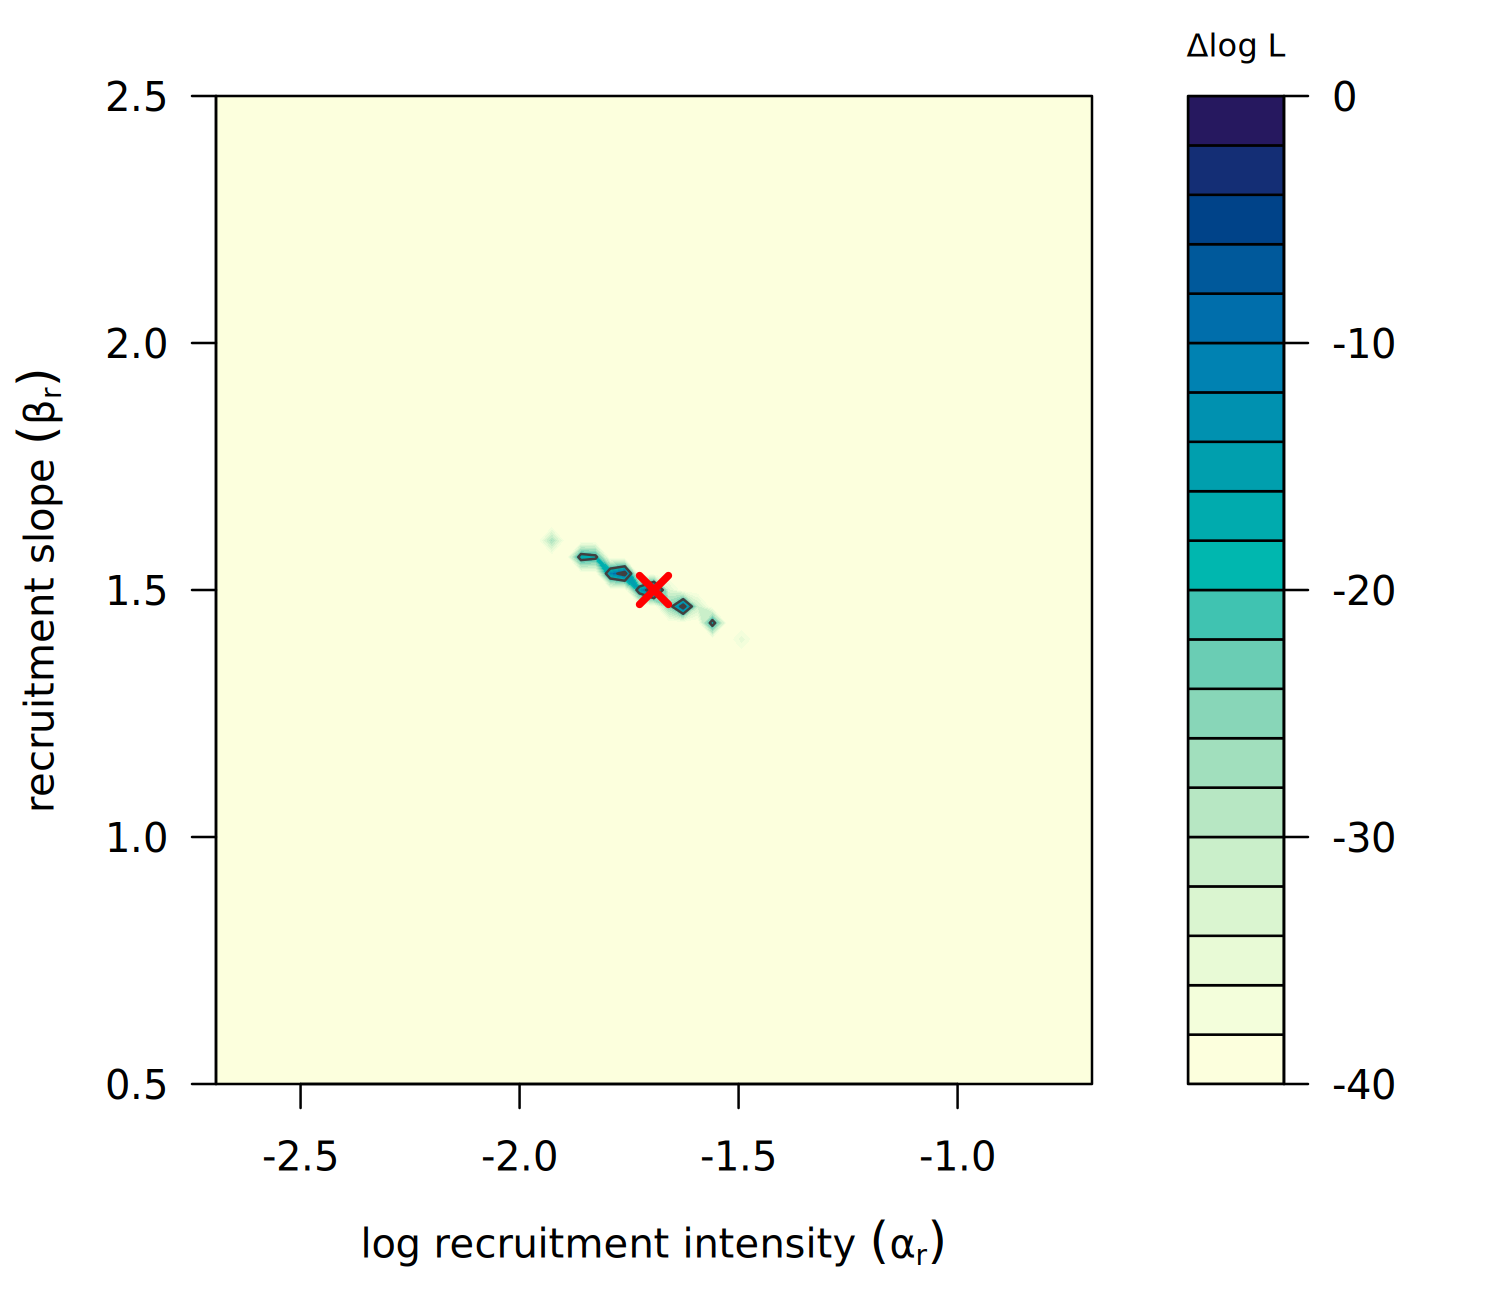
\includegraphics[width=0.7\textwidth]{confounding_ridge.png}
\caption{Relative profile log-likelihood over recruitment level $\alpha_r$ and
slope $\beta_r$, all other parameters at truth (red cross), capped at
$\Delta\log L=-40$ to reveal structure. The likelihood is sharply peaked except
along a thin ridge oriented in the negative-correlation direction: the
non-identified recruitment direction.}
\label{fig:ridge}
\end{figure}

\subsection{Excitation restores recruitment identifiability}
\label{sec:sim-excite}
Proposition~\ref{prop:excite} predicts that the confounding stems from
near-stationarity and should weaken as the population is perturbed off its stable
distribution. We tested this with matched data sets differing only in the initial
state, interpolated from exactly the stable distribution $\mathbf{w}$ to a strong
small-size cohort pulse, holding the vital rates, population size, and observation
noise fixed (Figure~\ref{fig:excitation}). Three patterns emerge. First, the
dominant eigenvalue $\lambda$ is recovered essentially perfectly at \emph{every}
excitation level (relative error $<0.01$), including at exact stationarity---the
asymptotic functional is identified even when the rates are not, the positive half
of Proposition~\ref{prop:excite}. Second, survival remains identified throughout
(contraction $\approx 0.98$). Third, recruitment intensity---nearly unrecoverable
near stationarity (relative error $\approx 0.8$--$1.1$, level/slope posterior
correlation below $-0.99$)---is progressively recovered as excitation increases,
reaching relative error $0.03$ and level/slope correlation $-0.31$ under the
strongest cohort pulse. The confounding is thus \emph{excitation-limited}: a
perturbed population (following a disturbance, a strong cohort, or environmental
forcing) carries the temporal information needed to separate recruitment from
survival-growth, whereas one observed near equilibrium does not. This converts the
negative identifiability result into concrete design guidance---to recover
recruitment from size profiles, observe the population away from its stable
distribution.

\begin{figure}[H]
\centering
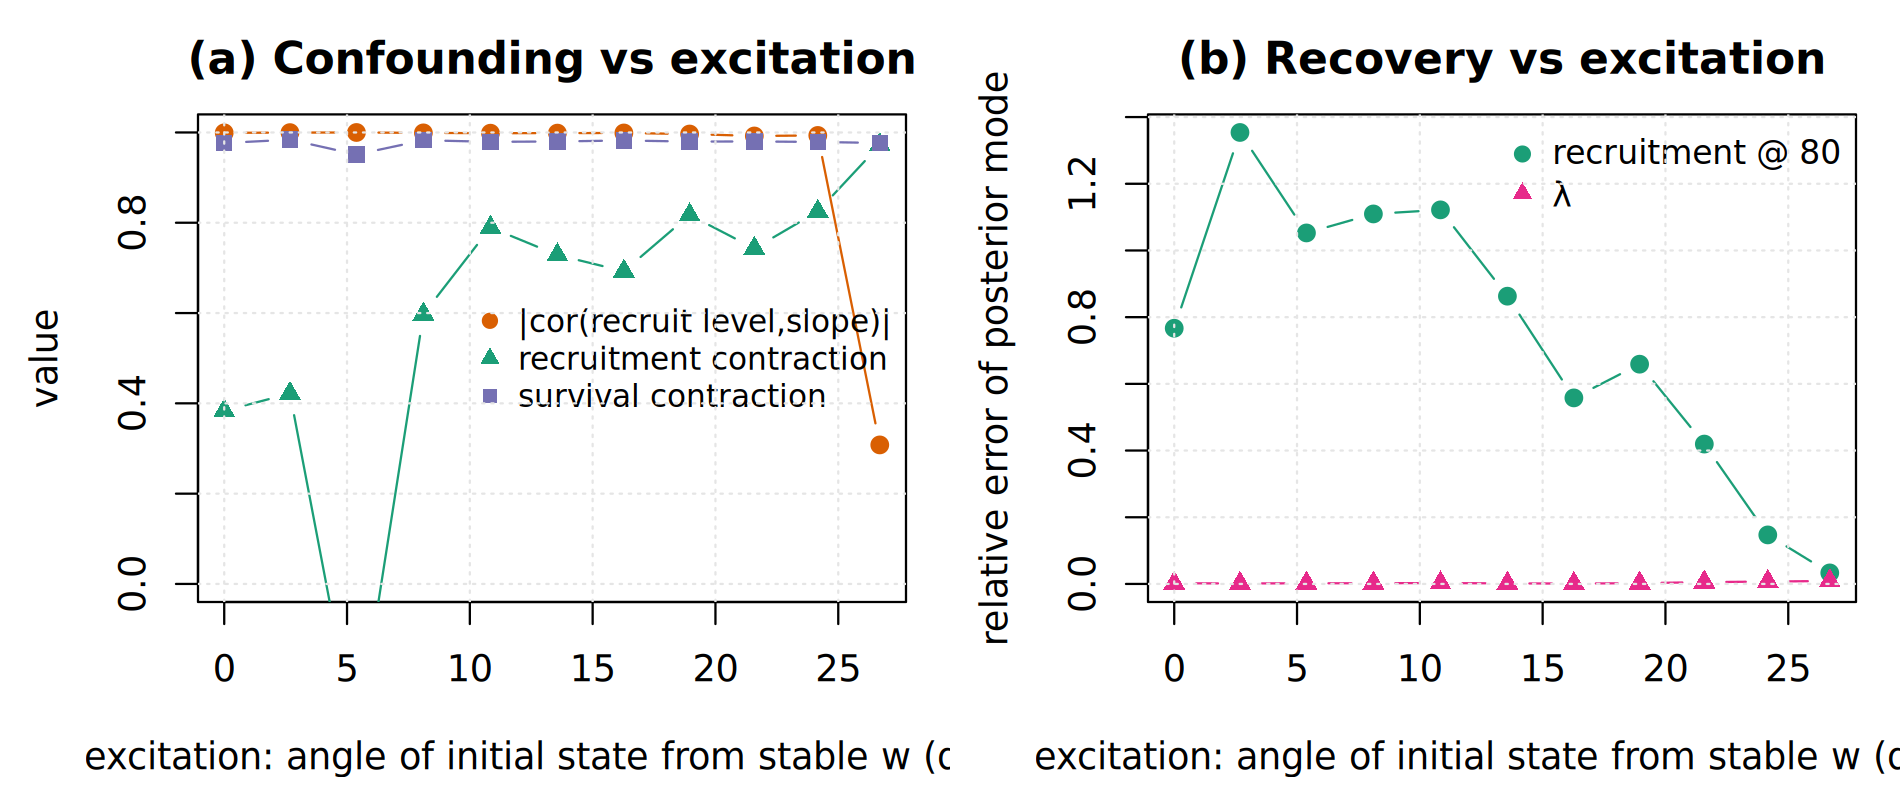
\includegraphics[width=\textwidth]{excitation.png}
\caption{Excitation experiment. As the initial state is perturbed further from
the stable distribution (x-axis: angle from $\mathbf{w}$): (a) the recruitment
level/slope confounding breaks and recruitment contraction rises, while survival
stays identified; (b) recruitment intensity recovery improves by an order of
magnitude, while $\lambda$ is recovered accurately at all excitation levels.}
\label{fig:excitation}
\end{figure}

\subsection{Broad recovery grid}
\label{sec:sim-grid}
A factorial Monte Carlo grid varied the allocation of a fixed 12-transition
budget ($1\times12$, $3\times4$, $6\times2$), initial population size, profile
detection, initial profile shape, and recovery likelihood (Poisson vs.\
Gamma--Poisson), producing 240 simulated datasets and 480 fits. Replicated short
trajectories outperformed one long trajectory on average
(Table~\ref{tab:design}), but no design achieved nominal coverage for all
quantities. Crucially, recovery was highly quantity-dependent
(Figure~\ref{fig:cov-quantity}): the recruit-size distribution, survival, and
mean growth were recovered well, whereas recruitment intensity and the dominant
eigenvalue were biased and overconfident---the simulation counterpart of the
ridge in Section~\ref{sec:sim-confound}.

\begin{table}[H]
\centering
\caption{Mean 95\% interval coverage by allocation of the 12-transition budget.}
\label{tab:design}
\small
\begin{tabular}{lcccc}
\toprule
Design & Poisson params & Poisson derived & GP params & GP derived\\
\midrule
$1\times12$ & 0.734 & 0.701 & 0.764 & 0.718\\
$3\times4$  & 0.795 & 0.775 & 0.818 & 0.818\\
$6\times2$  & 0.795 & 0.813 & 0.816 & 0.836\\
\bottomrule
\end{tabular}
\end{table}

\begin{figure}[H]
\centering
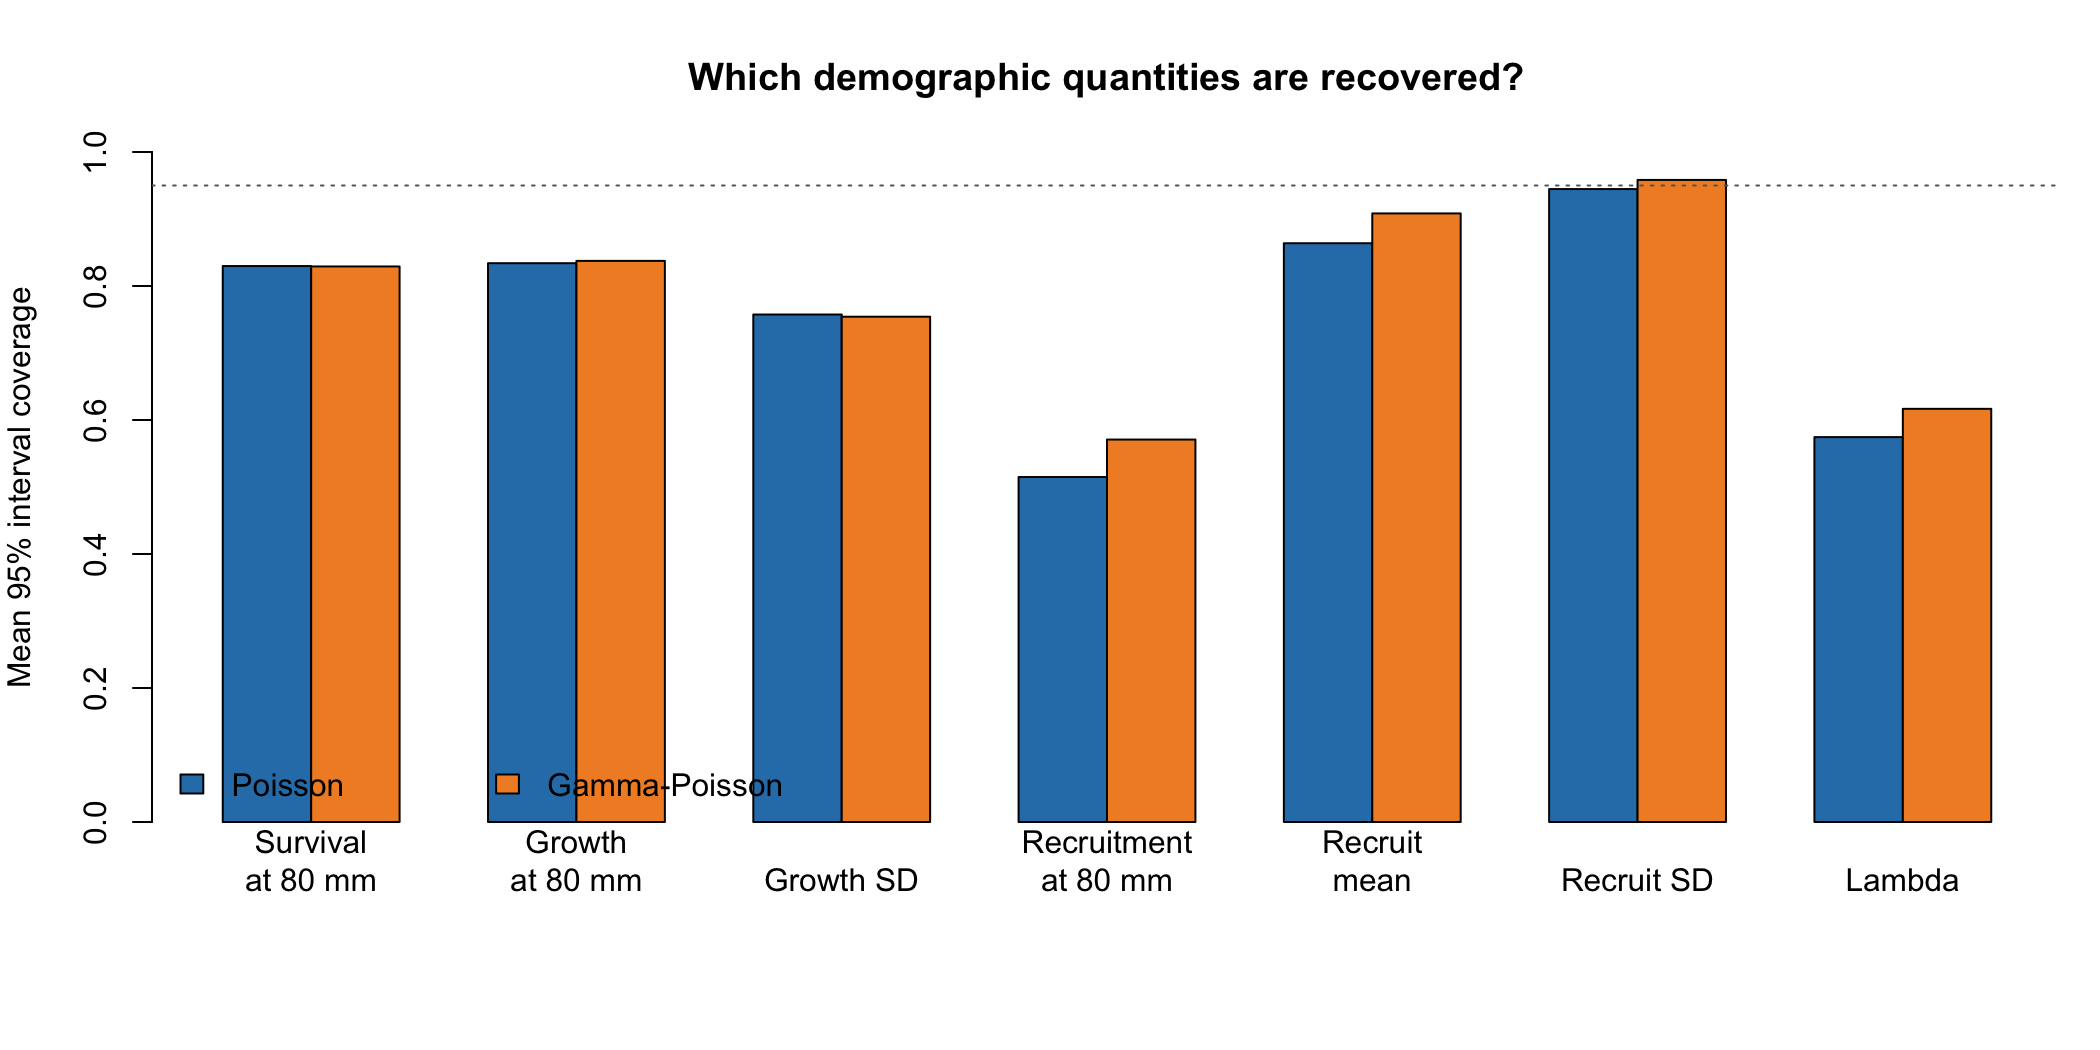
\includegraphics[width=0.85\textwidth]{monte_carlo/coverage_by_quantity.png}
\caption{Interval coverage varied sharply among demographic quantities. Recruit
size, survival, and mean growth were recovered more reliably than recruitment
intensity and the dominant eigenvalue.}
\label{fig:cov-quantity}
\end{figure}

\subsection{Calibration of the posterior approximation}
\label{sec:sim-sbc}
We validated the Laplace posterior by simulation-based calibration, generating
data from the recovery model's own data-generating process so that rank
non-uniformity isolates computational and approximation error rather than
misspecification (Figure~\ref{fig:sbc}). Under an informative prior, 200 of 200
fits succeeded and 10 of 11 parameters had uniform rank statistics
(only the overdispersion parameter $\log\phi$ was mildly miscalibrated). Under a
diffuse prior the rank histograms became U-shaped---posterior intervals
overconfident---most severely along exactly the confounded recruitment and growth
directions. The practical implication is that, under diffuse priors, interval
inference for the confounded directions should come from full posterior sampling
rather than the Gaussian approximation.

\begin{figure}[H]
\centering
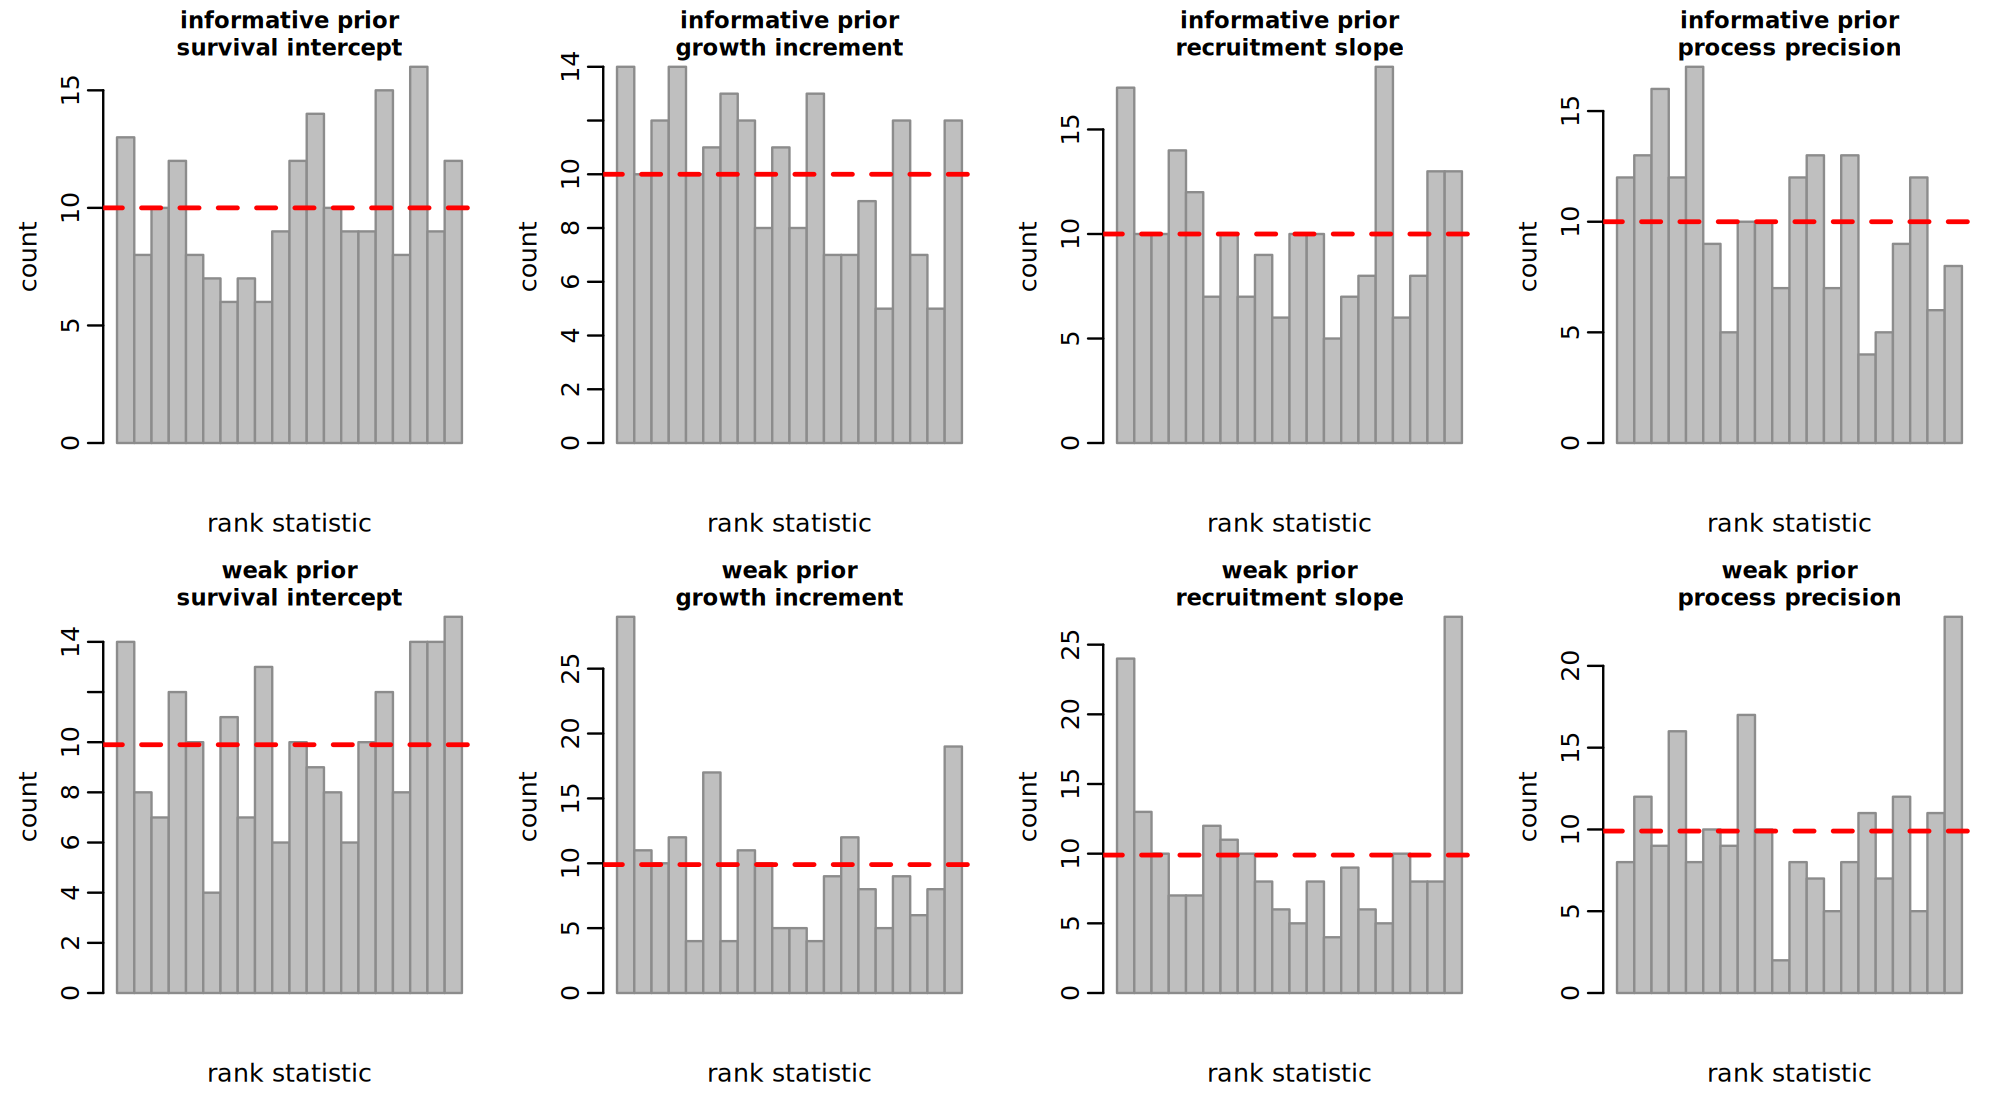
\includegraphics[width=\textwidth]{sbc_ranks.png}
\caption{Simulation-based calibration rank histograms (dashed line: uniform
expectation). Top: informative prior, ranks approximately uniform. Bottom:
diffuse prior, U-shaped ranks indicating overconfident intervals, worst for the
recruitment slope.}
\label{fig:sbc}
\end{figure}

\subsection{Observation-model robustness}
\label{sec:sim-detect}
A constant, size-independent detection probability is absorbed by the linear
projection and does not bias the profile-only fit. Size-dependent detection does.
We simulated three regimes---constant detection, unknown time-varying effort, and
size-dependent detection---and fit the standard recovery model
(Figure~\ref{fig:detect}). Under constant detection, survival-at-80 coverage was
0.90--0.95; under time-varying effort it fell to about 0.65; under
size-dependent detection it collapsed to zero, because a size-dependent change in
detectability is absorbed as demographic change. This is the dominant real-world
threat to profile-only inference and motivates the application caveats below.

\begin{figure}[H]
\centering
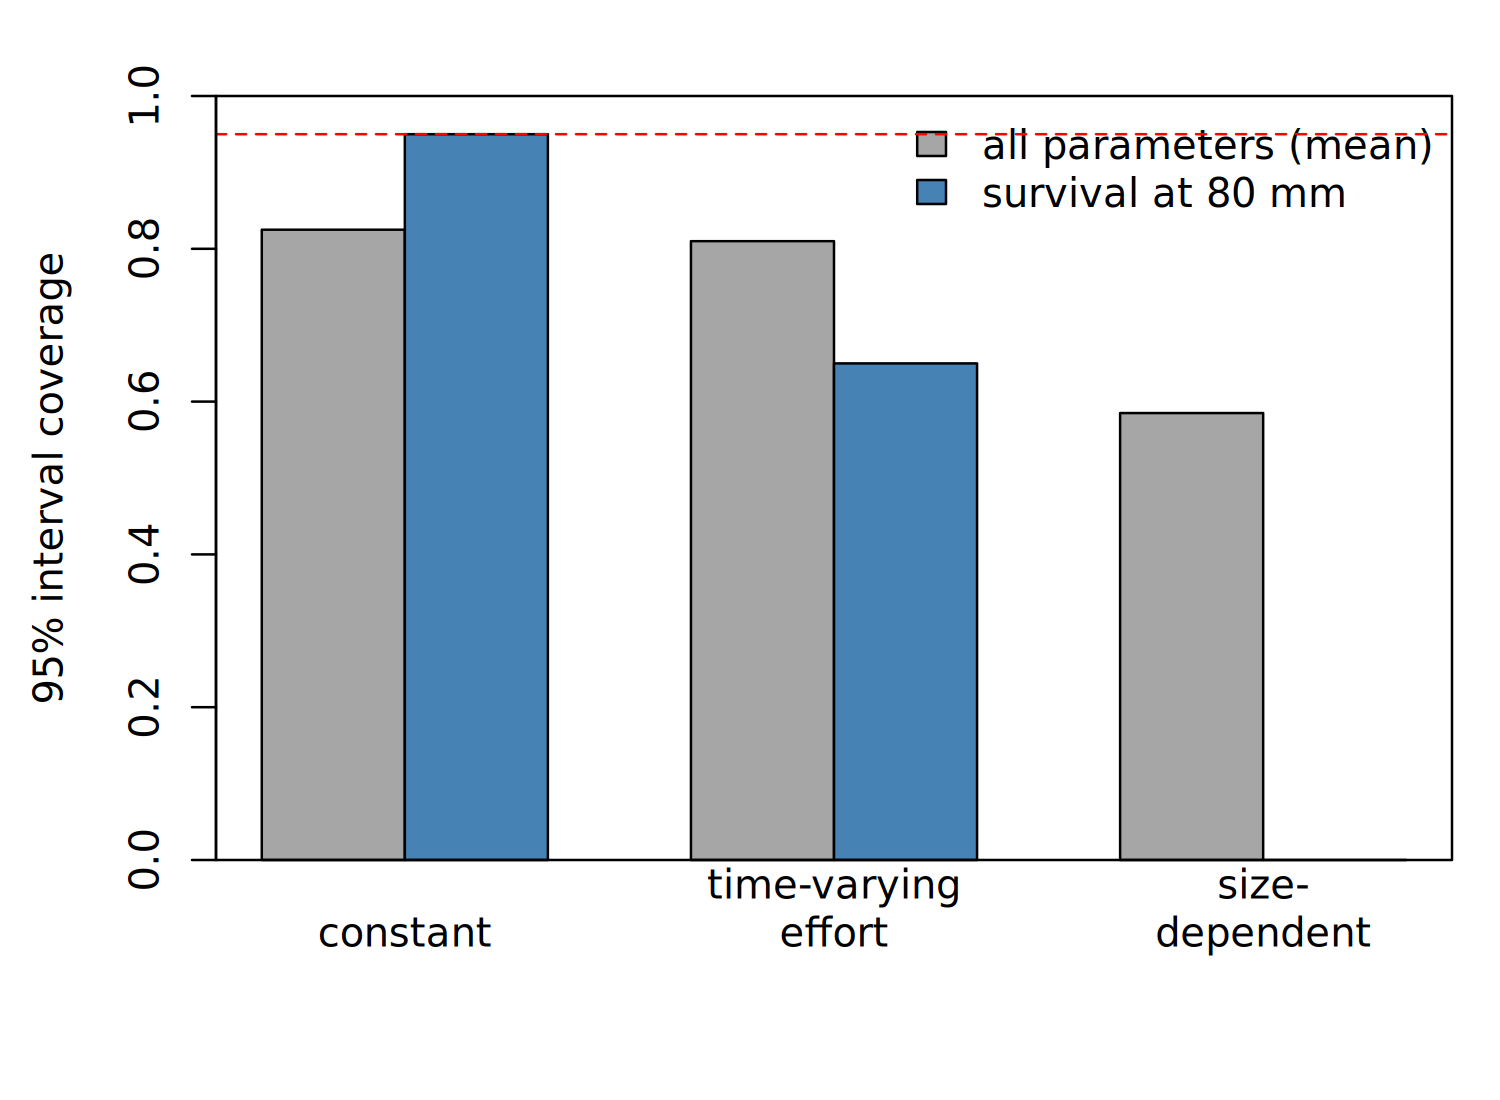
\includegraphics[width=0.62\textwidth]{detection_robustness.png}
\caption{95\% interval coverage (Gamma--Poisson recovery) under three detection
regimes. Size-dependent detection collapses survival coverage; the dashed line is
the nominal 0.95 level.}
\label{fig:detect}
\end{figure}

\subsection{Auxiliary data and transportability}
\label{sec:sim-aux}
Because recruitment intensity is the least identified rate, we quantified how much
external individual-level fecundity information resolves it, expressed as an
explicit auxiliary study of $n_e$ fish analyzed by Poisson regression whose
(approximate) posterior becomes the prior for $(\alpha_r,\beta_r)$. Correctly
transportable external data improved recruitment recovery monotonically in $n_e$;
800 external fish cut recruitment-curve RMSE by about 70\% and raised
recruitment-at-80 coverage from 0.53 to 0.87. A precise but \emph{biased}
external study produced low point-estimate error yet zero coverage; robust
(mixture) borrowing mitigated but did not eliminate the damage, and could reject
a non-transportable study only when the conflict altered profile dynamics along a
likelihood-informed direction (Figure~\ref{fig:transport}). No single amount of
external-study bias is universally safe.

\begin{figure}[H]
\centering
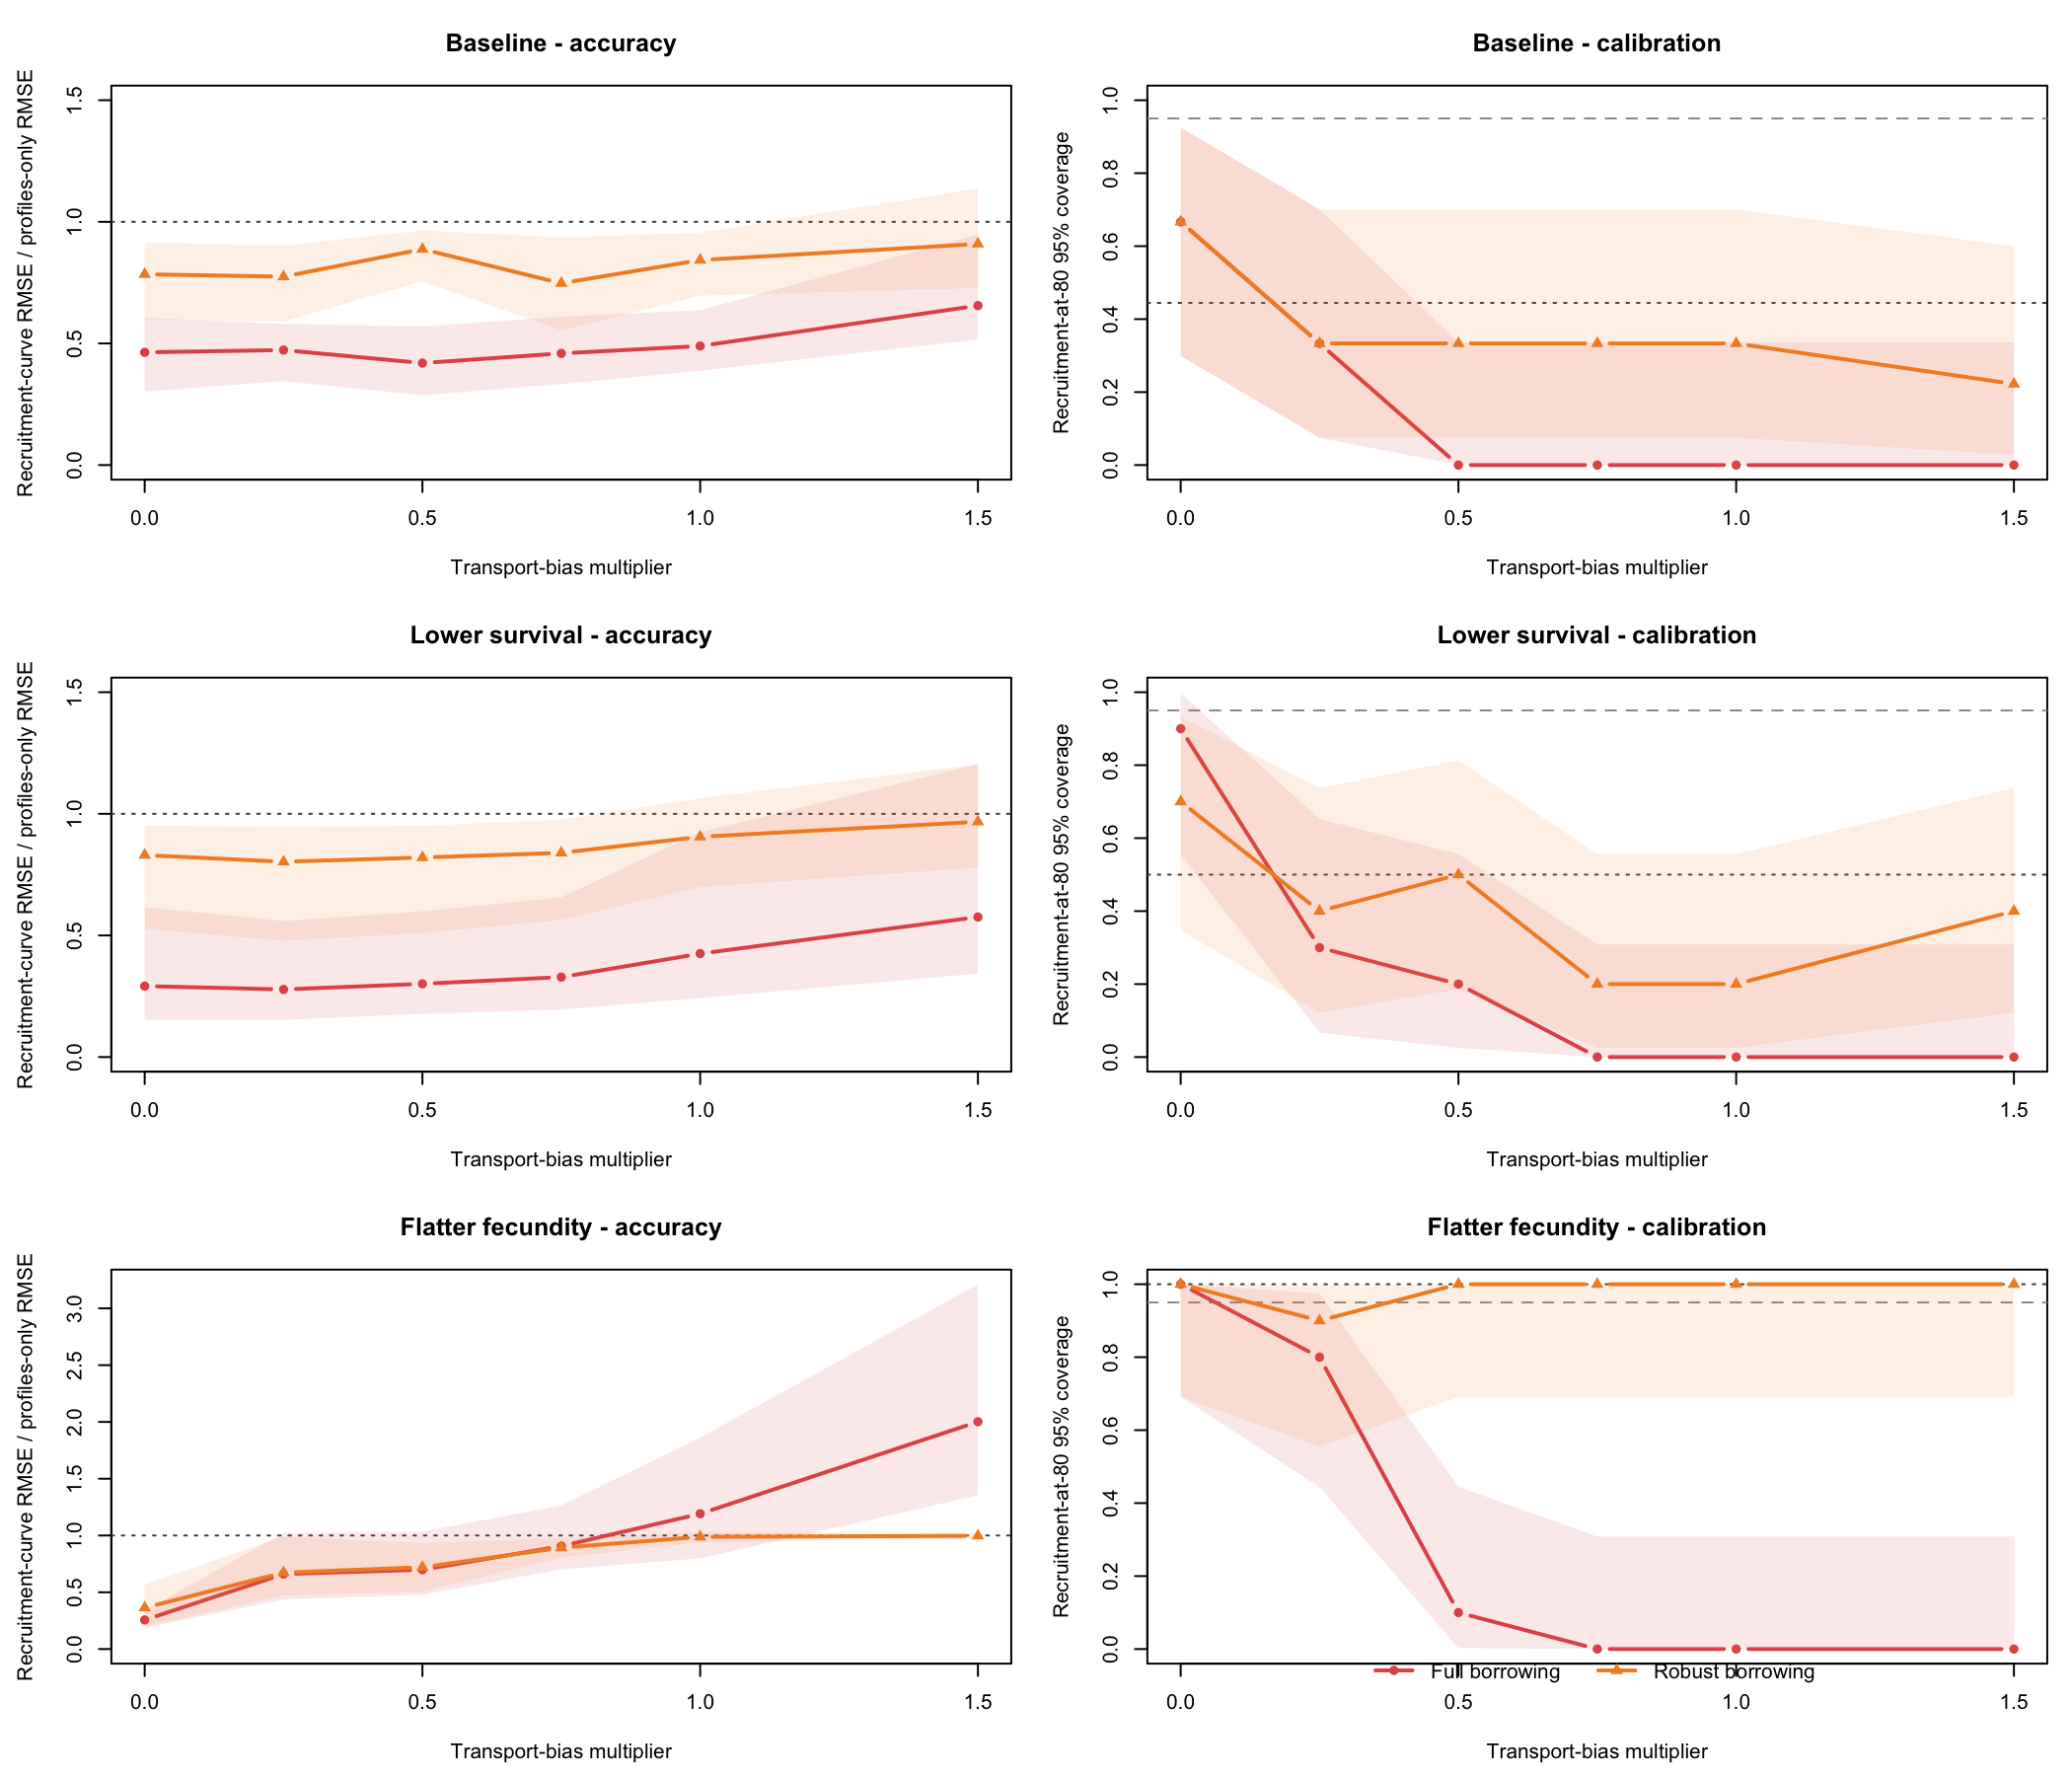
\includegraphics[width=\textwidth]{transportability_boundary/borrowing_safety_boundary.png}
\caption{Accuracy and calibration as external-study bias increases (pooled across
biological truths; 30 replicates per cell). Full borrowing improves point error
but loses calibration at the smallest tested bias; robust borrowing degrades more
gracefully. Dotted lines: profiles-only performance; dashed: nominal coverage.}
\label{fig:transport}
\end{figure}

\subsection{Paired-data benchmark}
\label{sec:sim-paired}
Finally, on 200 datasets each carrying both profiles and capture--recapture
histories, we compared profile-only, capture--recapture-only, integrated, and
complete-history oracle analyses (Figure~\ref{fig:paired}). Capture--recapture
efficiently identified survival and growth but carried essentially no information
about recruitment (its apparently perfect recruitment coverage reflected
prior-width intervals, not recovery). Integration improved point accuracy for
survival and growth but narrowed intervals below nominal, as residual
discrepancy between observed and deterministically projected profiles was
absorbed by other parameters---a caution we return to in the application.

\begin{figure}[H]
\centering
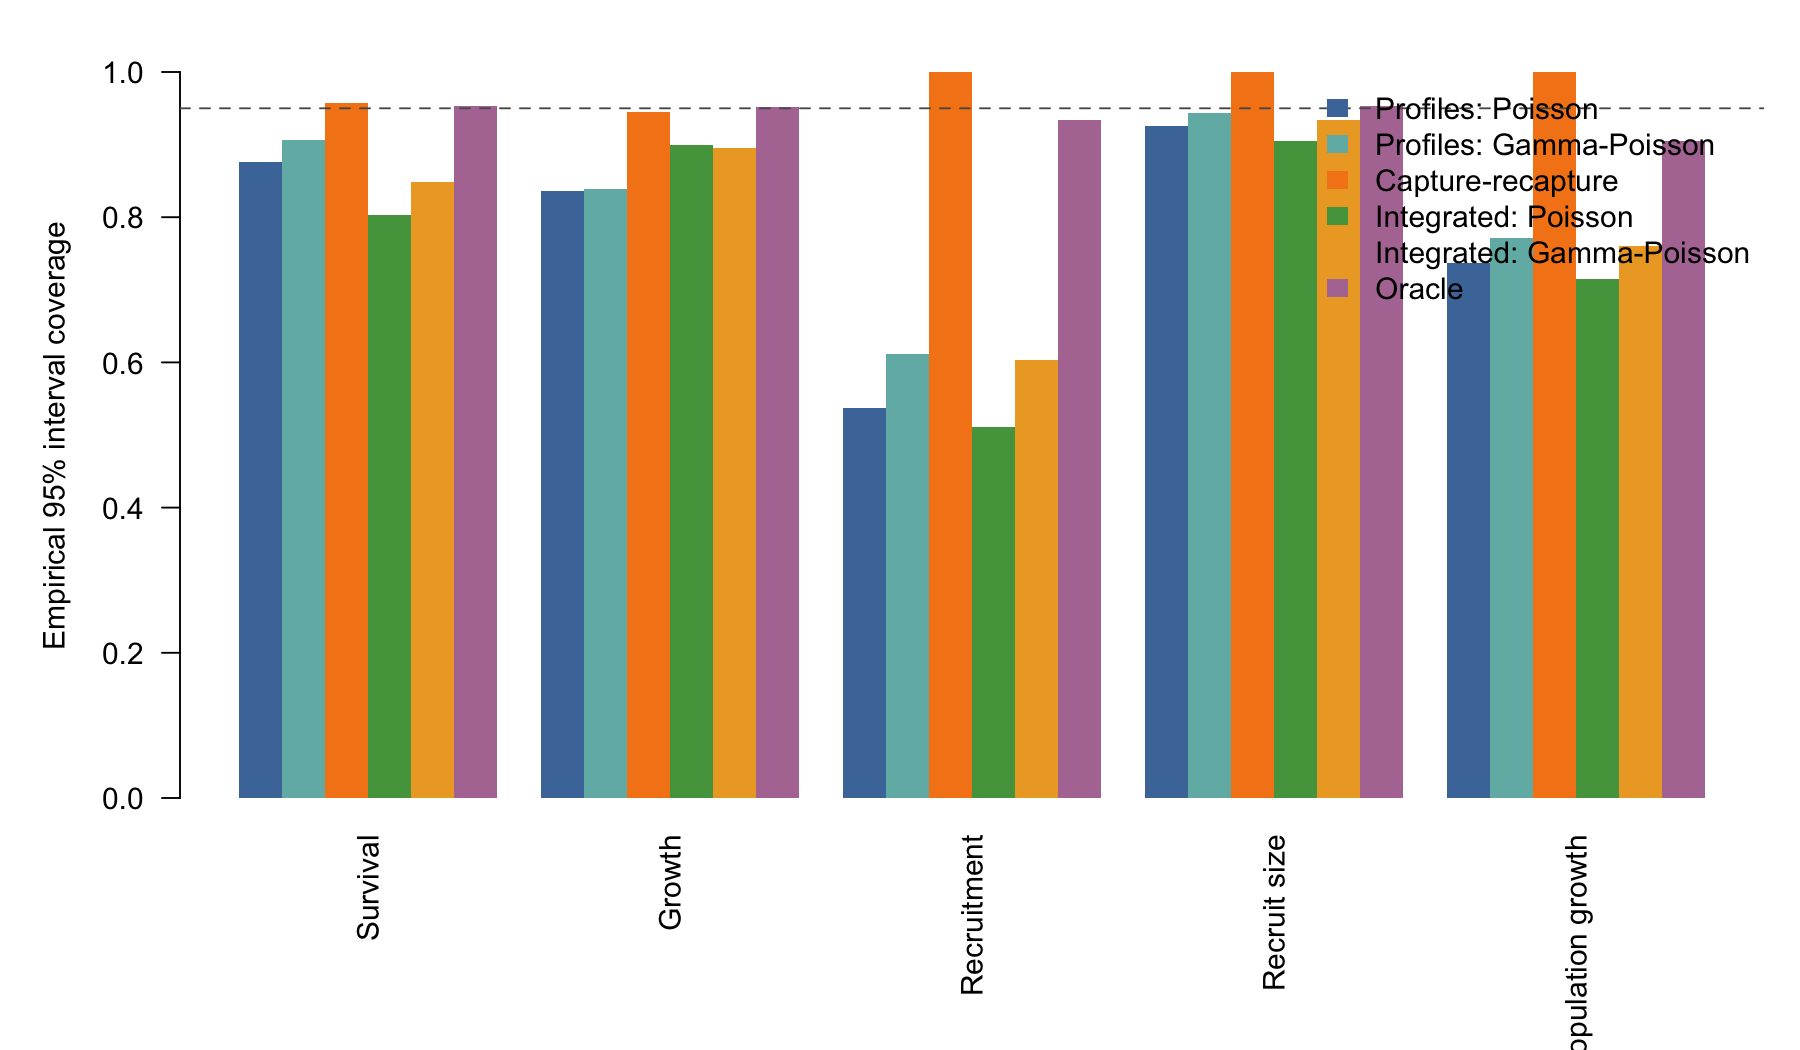
\includegraphics[width=0.85\textwidth]{paired_benchmark/coverage_by_data_source.png}
\caption{Empirical interval coverage in the paired-data benchmark. Perfect
capture--recapture coverage for recruitment and population growth reflects
prior-dominated wide intervals, not data-based identification.}
\label{fig:paired}
\end{figure}

\section{Application: West Brook Brook Trout}
\label{sec:app}

\subsection{Data and study system}
We applied the framework to a long-term passive-integrated-transponder (PIT)
tagging study of brook trout (\emph{Salvelinus fontinalis}) in the West Brook,
Massachusetts, USA \citep{letcher2015}, obtained from the U.S. Geological Survey
\citep{westbrookdata}. We treat the whole stream network (main stem and three
tributaries) as one population, because a non-trivial fraction of fish move
between reaches each year and a main-stem-only boundary would count emigrants as
deaths. The profile stream is the standardized seasonal size cross-section over
2000--2019 (20 annual occasions, 19 transitions), restricted to sizes
$\ge 70$~mm where electrofishing detection is approximately size-uniform;
recruitment is modeled as entry into this observable class. The size profiles are
close to stationary across the two decades (Figure~\ref{fig:wb-profiles}).

\needbio{Expand this into a proper study-system description: stream
characteristics, sampling design and electrofishing protocol, age/size structure
of brook trout in this system, the biological meaning of ``recruitment to the
$\ge 70$~mm class'' here, and why the population may be near a stable size
distribution. Add references to the field program.}

\begin{figure}[H]
\centering
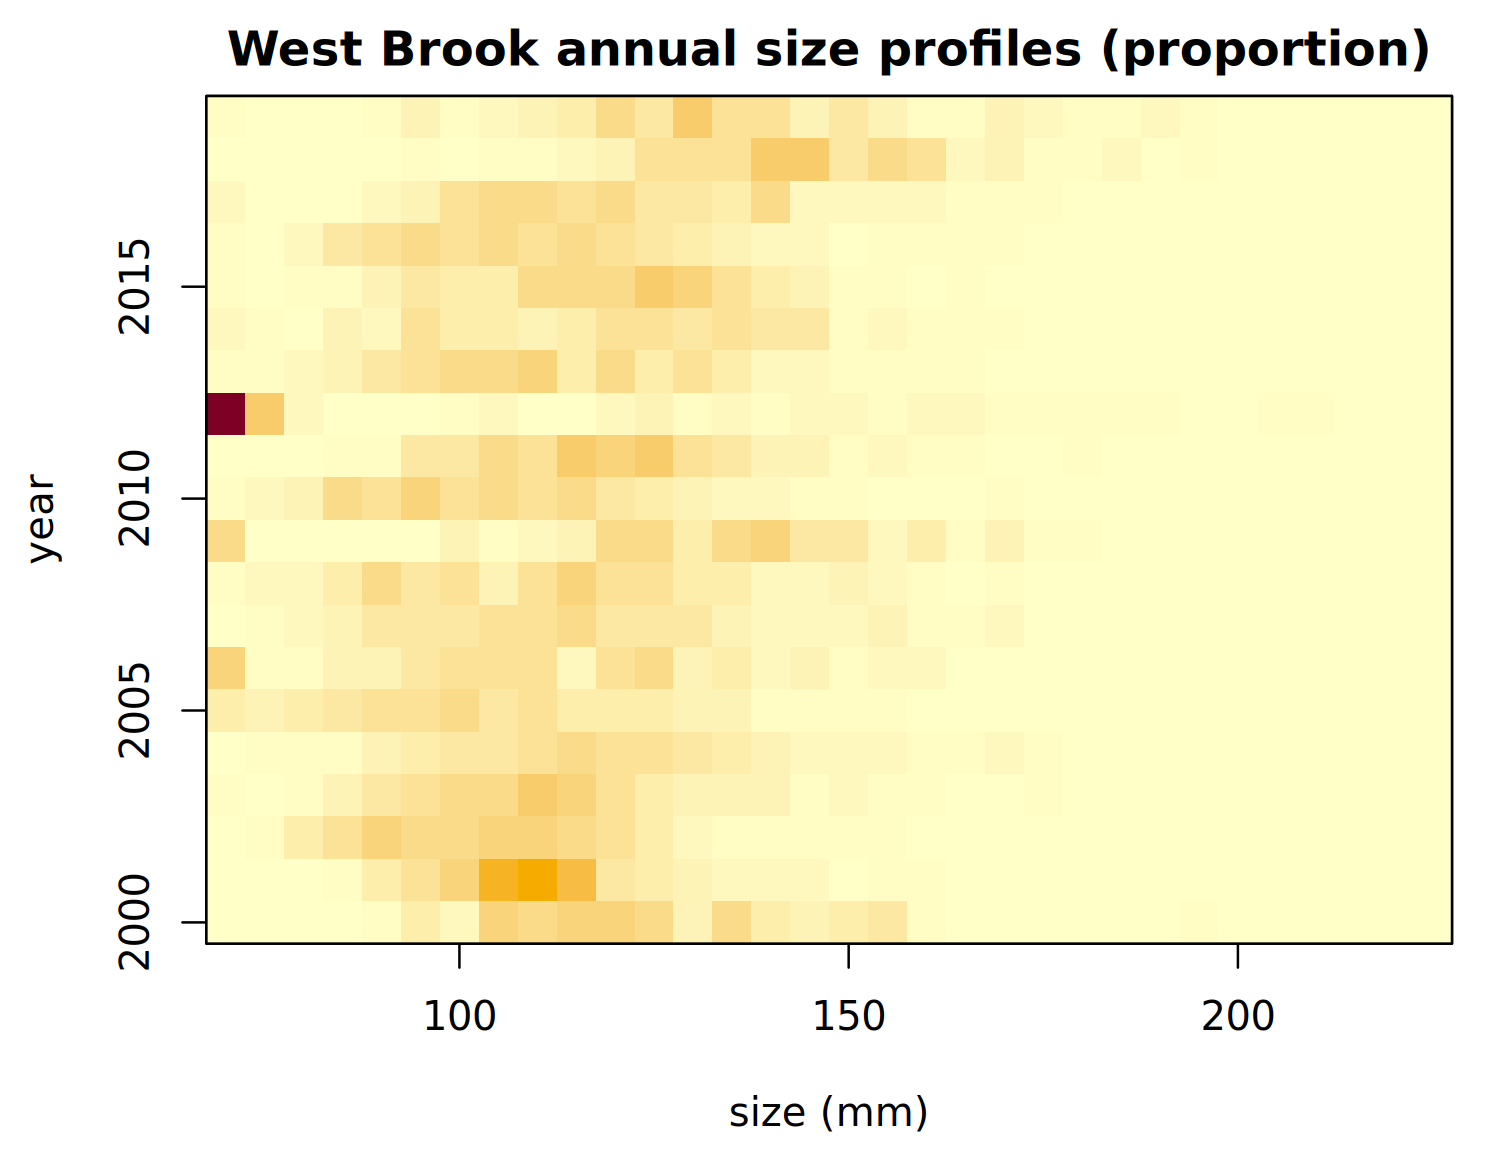
\includegraphics[width=0.6\textwidth]{west_brook_profiles.png}
\caption{Observed annual size profiles (proportion by 5\,mm bin) of West Brook
brook trout, 2000--2019. The distribution is close to stationary across years.}
\label{fig:wb-profiles}
\end{figure}

\subsection{Profile-only, mark--recapture, and integrated analyses}
We fit the profile-only inverse IPM, a size-structured mark--recapture model for
survival and growth (with detection estimated at $\hat p = 0.97$ from a
constant-rate Cormack--Jolly--Seber model over the full histories, 20{,}077
recapture events), and an integrated model combining both likelihoods. Growth
estimated from recaptures is detection-free and serves as the cleanest
cross-check.

The profile-only fit is internally plausible---moderate survival, positive
growth, $\lambda\approx 1$, a positive-definite posterior---yet it is contradicted
by the individual data on both quantities the recaptures can check
(Table~\ref{tab:wb}, Figure~\ref{fig:wb}). Profile-only inference
\emph{underestimates the growth increment} (12.6 vs.\ 32.3~mm\,yr$^{-1}$), the
signature of a near-stationary size distribution that hides how fast individuals
move through it, and \emph{misses the size gradient in apparent survival}
(roughly flat near 0.44, versus a clear decline from 0.31 to 0.12 with size in the
recapture and integrated analyses, reflecting greater emigration of larger fish).
Recruitment intensity remains unidentified by profiles (level/slope posterior
correlation $-0.995$), as in the simulations. The integrated analysis adopts the
recapture survival and growth and tightens the population growth rate to
$\lambda = 1.016\,[1.00, 1.05]$.

\begin{table}[H]
\centering
\caption{West Brook brook trout: posterior median [95\% interval] by analysis.
Mark--recapture survival is \emph{apparent} survival, which folds in
size-dependent emigration from the network.}
\label{tab:wb}
\small
\begin{tabular}{lccc}
\toprule
Quantity & Profile-only & Mark--recapture & Integrated\\
\midrule
Survival @ 80 mm  & 0.43 [0.29, 0.60] & 0.31 [0.31, 0.32] & 0.31 [0.31, 0.32]\\
Survival @ 110 mm & 0.45 [0.35, 0.55] & 0.20 [0.20, 0.21] & 0.20 [0.19, 0.21]\\
Survival @ 140 mm & 0.46 [0.34, 0.58] & 0.12 [0.12, 0.13] & 0.12 [0.11, 0.12]\\
Growth incr.\ @ 80 mm & 12.6 [9.3, 15.6] & 32.3 [31.7, 32.8] & 32.1 [31.5, 32.7]\\
$\lambda$ & 0.99 [0.97, 1.11] & --- & 1.016 [1.00, 1.05]\\
\bottomrule
\end{tabular}
\end{table}

\begin{figure}[H]
\centering
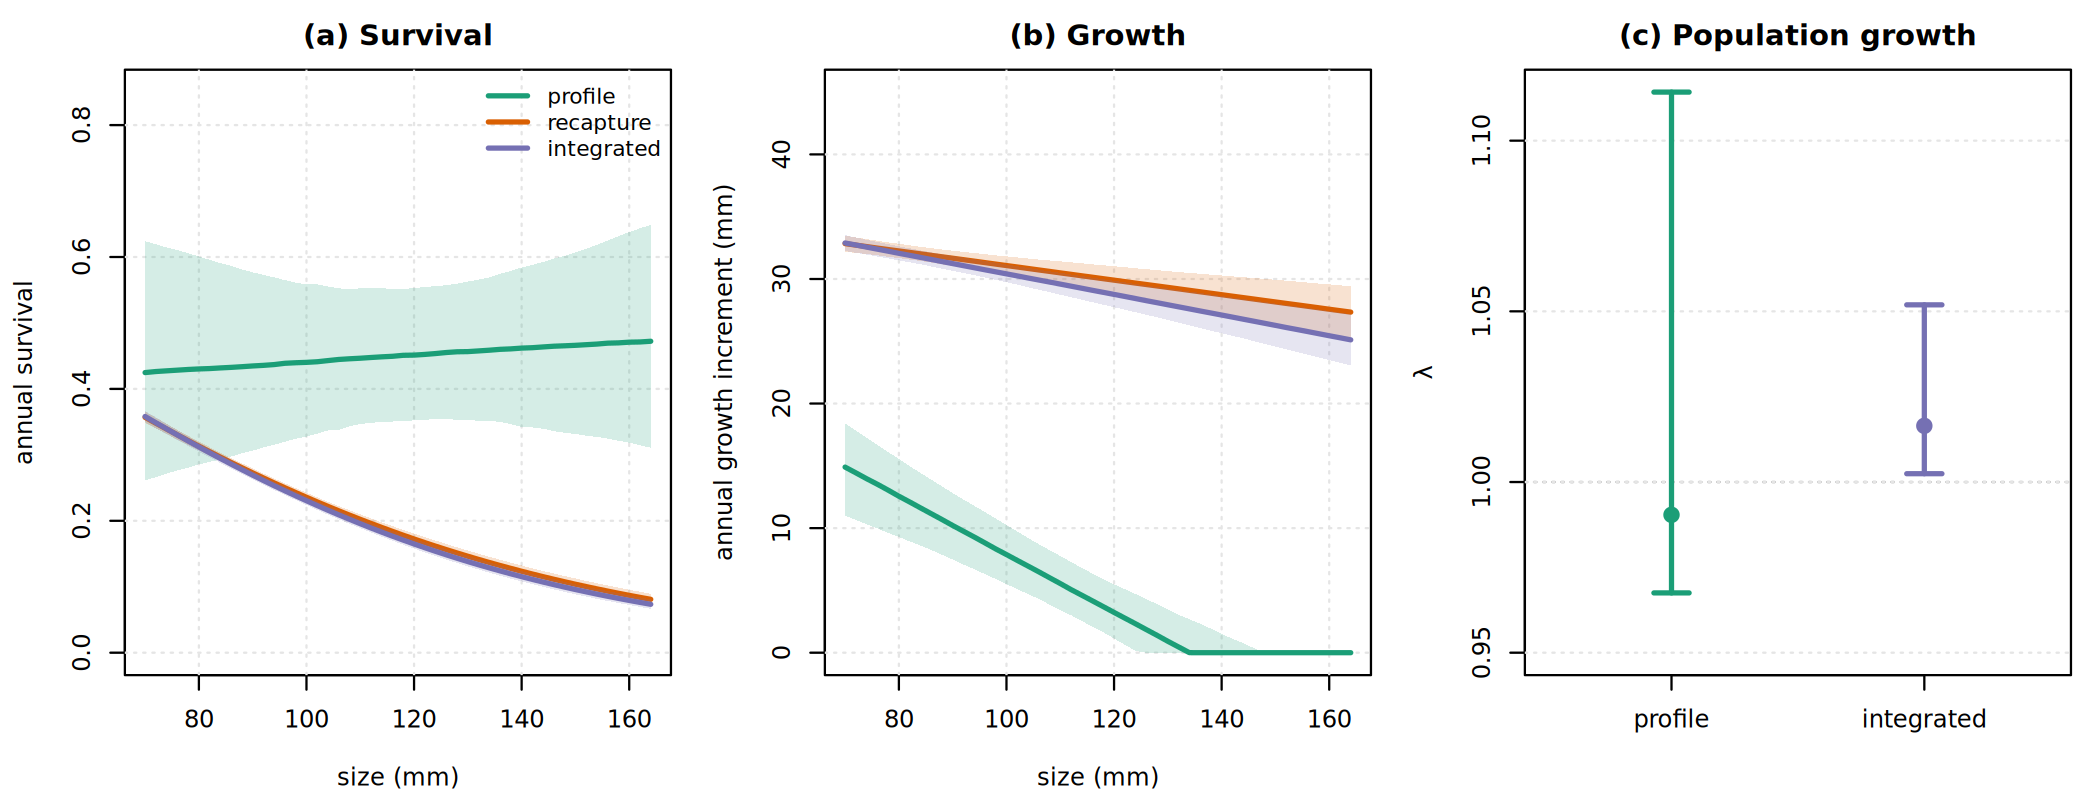
\includegraphics[width=\textwidth]{west_brook_comparison.png}
\caption{West Brook brook trout: (a) survival, (b) growth increment, and (c)
population growth $\lambda$ under profile-only, mark--recapture, and integrated
analyses (medians with 95\% bands/intervals). The profile-only fit underestimates
growth and misses the survival size gradient that the individual data reveal.}
\label{fig:wb}
\end{figure}

\needbio{Biological interpretation of these contrasts: is the $\sim$32\,mm\,yr$^{-1}$
recapture growth consistent with known brook trout growth in this system? Is the
declining apparent survival with size attributable to emigration of larger fish,
size-selective mortality, or both? What would the management or ecological
reading of the profile-only versus integrated $\lambda$ be? Please also confirm
the framing of the size-dependent-detection caveat for electrofishing.}

\subsection{Profile-only uncertainty is multimodal and concentrates on an
iso-$\lambda$ manifold}
\label{sec:app-mcmc}
Replacing the Laplace approximation with full MCMC (four adaptive-Metropolis
chains) exposes the non-identifiability directly. The chains do \emph{not}
converge on the vital rates (split $\widehat R$ up to $6.6$); this is not a
sampler failure but a property of the target. The chains settle in biologically
distinct regimes---survival at 80\,mm from $0.005$ to $0.12$, growth increment
from $3$ to $14$\,mm, recruitment over more than an order of magnitude---that all
reproduce the near-stationary profiles of Figure~\ref{fig:wb-profiles}. Yet
across the pooled posterior the dominant eigenvalue varies by only 2.5\%
(coefficient of variation), versus 222\% for survival at 80\,mm and 131\% for
recruitment intensity (Figure~\ref{fig:manifold}): a direct, real-data instance
of Proposition~\ref{prop:excite}. The Laplace mode (survival $\approx 0.43$) does
not lie where the posterior mass concentrates, so its narrow intervals for the
confounded directions are not trustworthy. We therefore report $\lambda$ as the
profile-identified functional and treat profile-only vital-rate point estimates
as non-identified absent individual data; the integrated analysis both resolves
the rates and shifts $\lambda$ to $1.016\,[1.00,1.05]$.

\begin{figure}[H]
\centering
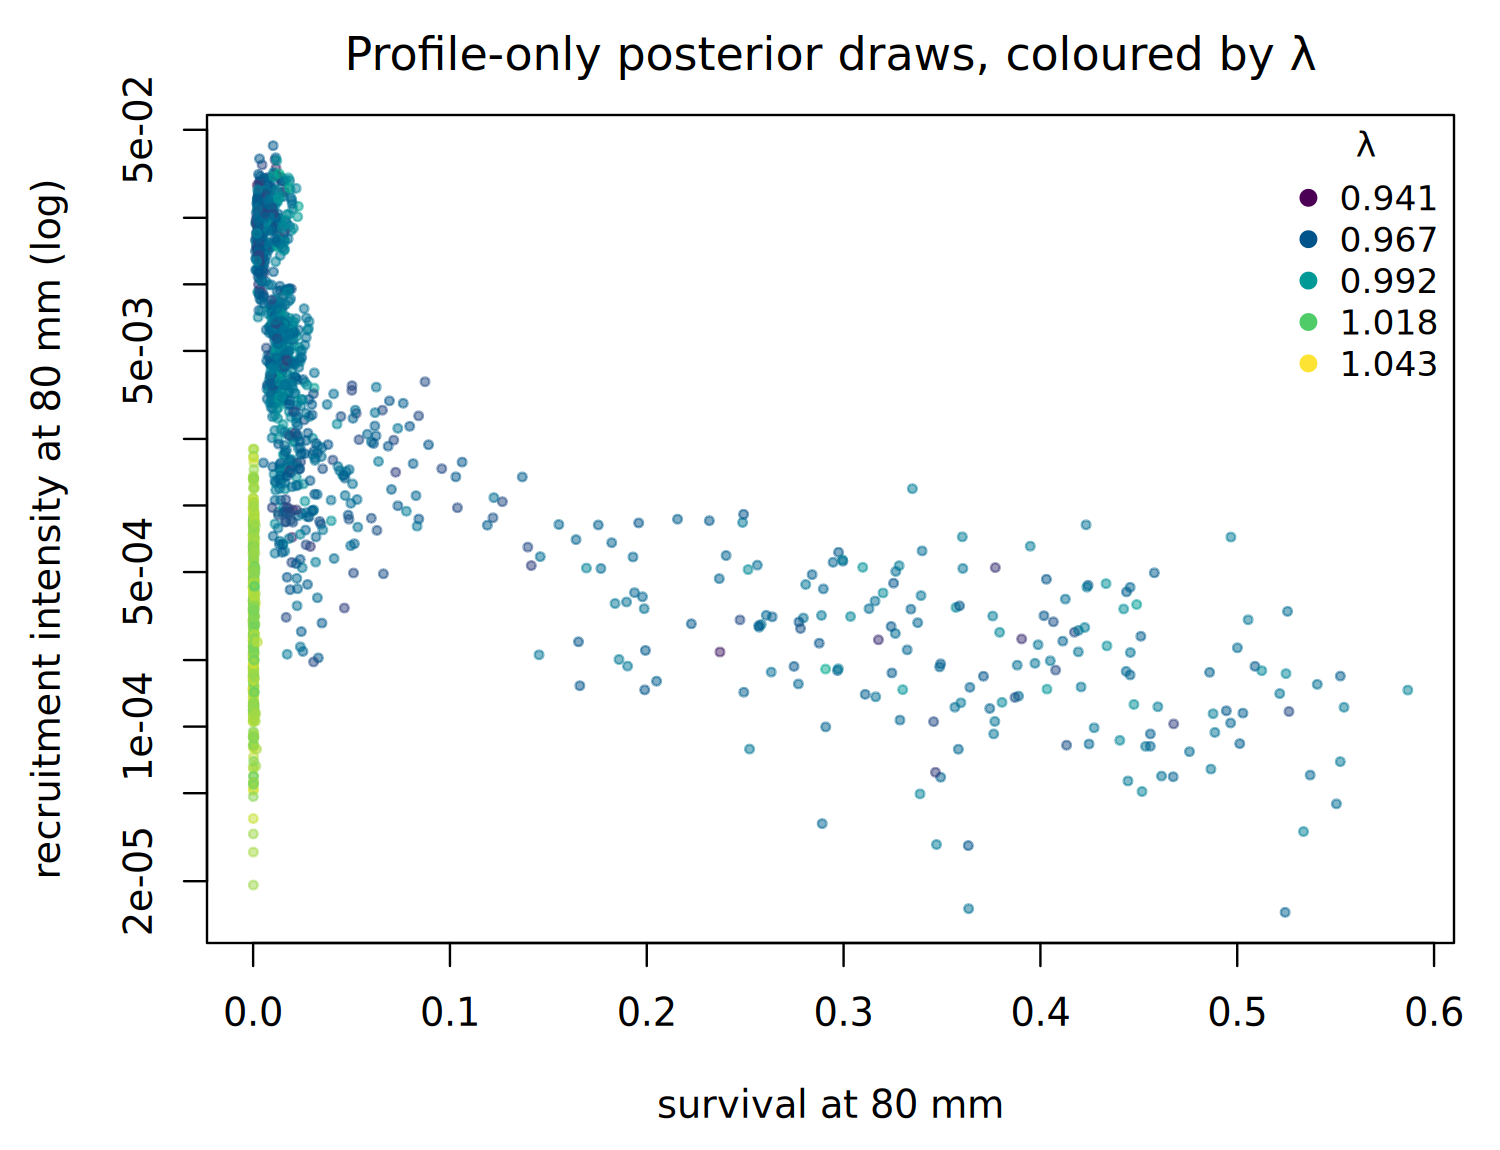
\includegraphics[width=0.6\textwidth]{identified_manifold.png}
\caption{Profile-only posterior draws (West Brook brook trout) in the
survival--recruitment plane, coloured by the implied dominant eigenvalue
$\lambda$. Biologically very different vital-rate combinations span the plane,
yet $\lambda$ varies little (CV 2.5\% vs.\ 222\% for survival): profiles identify
the asymptotic functional, not the rates that generate it.}
\label{fig:manifold}
\end{figure}

This non-identification is invisible to local diagnostics. The observed Fisher
information at the Laplace mode spans seven orders of magnitude, and nine of the
eleven information eigen-directions contract by more than half from the prior
(Figure~\ref{fig:subspace}); the single flat direction there is the recruit-size
location, unconstrained only because recruitment into the window is near zero at
that mode. A Hessian- or Laplace-based identifiability check would therefore
declare the model essentially identified, even though the global posterior is the
multimodal iso-$\lambda$ manifold of Figure~\ref{fig:manifold}. Local curvature
certifies practical identifiability \emph{at a point}; establishing global
identifiability requires manifold-revealing MCMC, profile likelihoods, or data
cloning.

\begin{figure}[H]
\centering
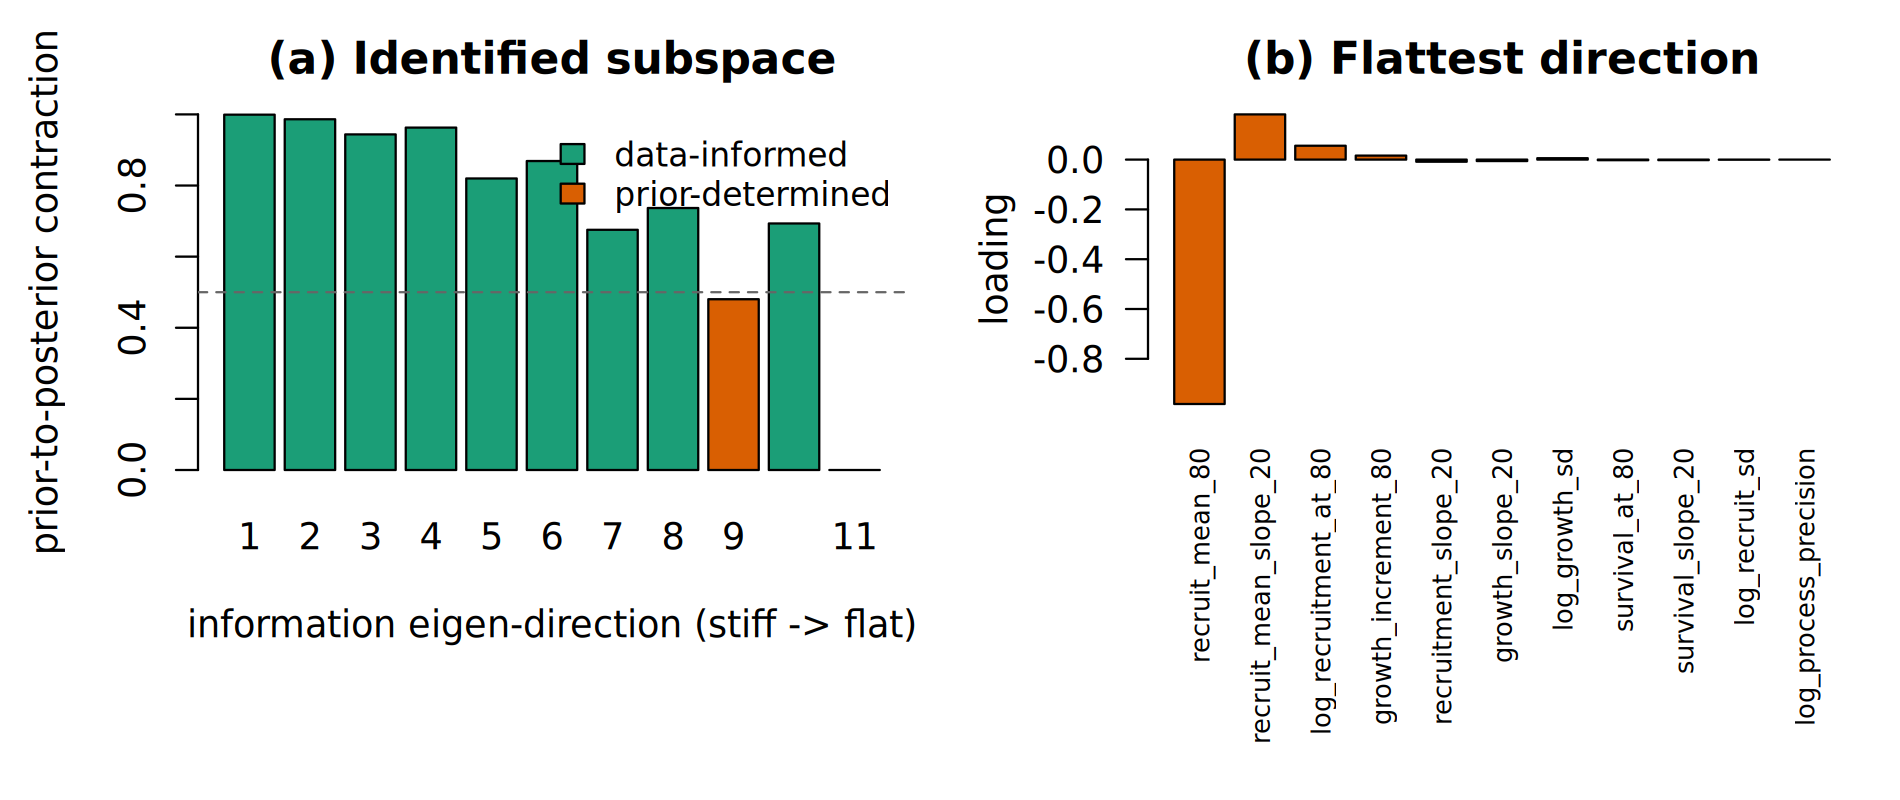
\includegraphics[width=\textwidth]{identified_subspace.png}
\caption{(a) Prior-to-posterior contraction along the observed-information
eigen-directions at the West Brook profile-only mode; nine of eleven exceed 0.5,
suggesting local identifiability. (b) The flattest direction loads almost
entirely on recruit-size location. Local curvature does not reveal the global
non-identification of Figure~\ref{fig:manifold}.}
\label{fig:subspace}
\end{figure}

\section{Discussion}
\label{sec:discussion}

Repeated size profiles are genuinely informative about some vital rates---survival,
the growth distribution, and recruit size---and almost uninformative about others,
chiefly recruitment intensity and, through it, the asymptotic growth rate. The
confounding is structural (a ridge that trades recruitment level against its size
gradient), it is sharpened by short series and near-stationary distributions, and
it is easily masked by an informative prior or by unmodeled size-dependent
detection. The brook trout application makes the practical stakes concrete: a
profile-only fit that passes every internal check still misstates growth by a
factor of two and inverts the survival size pattern, errors visible only against
individual data.

For practice we recommend: declaring the estimand before fitting; reporting
prior-to-posterior contraction and the recruitment level/slope correlation as
routine identifiability diagnostics; modeling, or at minimum bounding, size-
dependent detection; and expressing external information as an explicit,
transportability-checkable study design. Where individual data exist, an
integrated analysis is worth far more than its marginal cost, but its intervals
must be interpreted cautiously when the profile and individual components
disagree.

Limitations include reliance on a parametric vital-rate basis (flexible spline
bases are a direct extension), a closed-population deterministic projection
likelihood (the finite-population particle-filtered variant is developed
separately), and a single applied system. The framework and diagnostics, however,
are general to size- and stage-structured inverse problems.

\needbio{Two to three sentences on the ecological/management implications and on
how these recommendations would change analyses in your systems, plus any
domain-specific limitations we should acknowledge.}

\section*{Data and Code Availability}
The West Brook data are public domain (CC0) and available from the U.S.\
Geological Survey \citep{westbrookdata}; a fetch script is provided. All
simulation code, analysis scripts, and figure-generation code are in the project
repository.

\section*{Acknowledgments}
\needbio{Funding sources, field crews, and data-collection acknowledgments for
the West Brook program.}

\begin{thebibliography}{99}
\small
\bibitem[Cook et al.(2006)]{cook2006} Cook, S.R., Gelman, A., Rubin, D.B. (2006).
Validation of software for Bayesian models using posterior quantiles.
\emph{Journal of Computational and Graphical Statistics} 15, 675--692.

\bibitem[Easterling et al.(2000)]{easterling2000} Easterling, M.R., Ellner, S.P.,
Dixon, P.M. (2000). Size-specific sensitivity: applying a new structured
population model. \emph{Ecology} 81, 694--708.

\bibitem[Ellner and Rees(2006)]{ellner2006} Ellner, S.P., Rees, M. (2006).
Integral projection models for species with complex demography. \emph{The
American Naturalist} 167, 410--428.

\bibitem[Ghosh et al.(2012)]{ghosh2012} Ghosh, S., Gelfand, A.E., Clark, J.S.
(2012). Inference for size demography from point pattern data using integral
projection models. \emph{Journal of Agricultural, Biological, and Environmental
Statistics} 17, 641--677.

\bibitem[Gross et al.(2002)]{gross2002} Gross, K., Craig, B.A., Hutchison, W.D.
(2002). Bayesian estimation of a demographic matrix model from stage-frequency
data. \emph{Ecology} 83, 3285--3298.

\bibitem[Letcher et al.(2015)]{letcher2015} Letcher, B.H., Schueller, P., Bassar,
R.D., Nislow, K.H., Coombs, J.A., et al. (2015). Robust estimates of environmental
effects on population vital rates: an integrated capture--recapture model of
seasonal brook trout growth, survival and movement in a stream network.
\emph{Journal of Animal Ecology} 84, 337--352.

\bibitem[Merow et al.(2014)]{merow2014} Merow, C., Dahlgren, J.P., Metcalf,
C.J.E., Childs, D.Z., Evans, M.E.K., et al. (2014). Advancing population ecology
with integral projection models: a practical guide. \emph{Methods in Ecology and
Evolution} 5, 99--110.

\bibitem[Talts et al.(2018)]{talts2018} Talts, S., Betancourt, M., Simpson, D.,
Vehtari, A., Gelman, A. (2018). Validating Bayesian inference algorithms with
simulation-based calibration. \emph{arXiv:1804.06788}.

\bibitem[U.S. Geological Survey(2024)]{westbrookdata} U.S. Geological Survey
(2024). Passive integrated transponder tag data from the West Brook, MA, USA.
\emph{U.S. Geological Survey data release}, \doi{10.5066/P14PDHXM}.

\bibitem[Wood(1994)]{wood1994} Wood, S.N. (1994). Obtaining birth and mortality
patterns from structured population trajectories. \emph{Ecological Monographs}
64, 23--44.
\end{thebibliography}

\end{document}
